\documentclass{scrartcl}
\usepackage{graphicx}  % required for inserting images
\usepackage{float}

% for cyrillic and Bulgarian language
\usepackage[utf8]{inputenc}
\usepackage[T2A]{fontenc}
\usepackage[bulgarian]{babel}

% math packages
\usepackage{amsmath}
\usepackage{float}
\usepackage{amsfonts}
\usepackage{amssymb}

\usepackage{ragged2e}  % adds FlushLeft

\usepackage{listings}
\usepackage{xcolor}

\definecolor{codegreen}{rgb}{0,0.6,0}
\definecolor{codegray}{rgb}{0.5,0.5,0.5}
\definecolor{codepurple}{rgb}{0.58,0,0.82}
\definecolor{backcolour}{rgb}{0.95,0.95,0.92}

\lstdefinestyle{mystyle}{
    language=Octave,
    backgroundcolor=\color{backcolour},   
    commentstyle=\color{codegreen},
    keywordstyle=\color{magenta},
    numberstyle=\tiny\color{codegray},
    stringstyle=\color{codepurple},
    basicstyle=\ttfamily\footnotesize,
    breakatwhitespace=false,         
    breaklines=true,
    captionpos=b,
    keepspaces=false,                 
    %numbers=left,                    
    numbersep=5pt,
    showspaces=false,
    showstringspaces=false,
    showtabs=false,
    tabsize=2,
    basicstyle=\ttfamily\footnotesize,
    columns=fullflexible
}

\lstset{style=mystyle}

\title{Семинар 01}
\author{Ивайло Андреев}
\date{27 февруари 2025}

\begin{document}
\maketitle  % template title

\section{Въвеждаща задача}

\begin{FlushLeft}
Ще започнем със задача, давана на държавен изпит на специалност "Приложна математика", септември 2007г.
\end{FlushLeft}

\begin{FlushLeft}
Да се намери в явен вид функцията $f:(-\pi, 2\pi)\rightarrow\mathbb{R}$, определена от условията:
\end{FlushLeft}

$$
\begin{cases}
f'(x) = \dfrac{1}{\sin{x}+2\cos{x}+3}
\\
f(0) = 0
\end{cases}
$$

\begin{FlushLeft}
Ще намерим функцията в явен вид, като интегрираме
\end{FlushLeft}

$$f'(x) = \dfrac{1}{\sin{x}+2\cos{x}+3}$$

$$\displaystyle \int f'(x)\space dx = \int \dfrac{1}{\sin{x}+2\cos{x}+3} \space dx$$

$$\displaystyle \int \space df(x) = \int \dfrac{1}{\sin{x}+2\cos{x}+3} \space dx$$

\begin{align*}
\displaystyle f(x)
&= \int \dfrac{1}{\sin{x}+2\cos{x}+3} \space dx\\
&= \int \dfrac{1}{\dfrac{2\tan{(x/2)}}{1+\tan^2{(x/2)}}+\dfrac{2-2\tan^2{(x/2)}}{1+\tan^2{(x/2)}}+\dfrac{3+3\tan^2{(x/2)}}{1+\tan^2{(x/2)}}} \space dx\\
&\overset{u = x/2}{=} 2\int \dfrac{1+\tan^2{u}}{\tan^2{u}+2\tan{u}+5} \space du\\
&\overset{v=\tan{u}}{=} 2\int \dfrac{1+v^2}{v^2+2v+5} \space d\arctan{v}\\
&= 2\int \dfrac{1}{1+v^2}\dfrac{1+v^2}{v^2+2v+5} \space dv\\
&= 2\int \dfrac{1}{v^2+2v+1+4} \space dv\\
&= 2\int \dfrac{1}{(v+1)^2+4} \space dv\\
&= \dfrac{2}{4}\int \dfrac{1}{\dfrac{(v+1)^2}{4}+1} \space dv\\
&= \int \dfrac{1}{1+\left(\frac{v+1}{2}\right)^2} \space d\left(\frac{v+1}{2}\right)^2\\
&= \arctan{\left(\dfrac{v+1}{2}\right)} + C\\
&= \arctan{\left(\dfrac{\tan{\frac{x}{2}}+1}{2}\right)} + C
\end{align*}

\begin{FlushLeft}
Така намерихме $f$ в явен вид с точност до 1 произволна константа.
От даденото допълнително условие ще елиминираме константата.
\end{FlushLeft}

$$f(0) = 0 \implies \arctan{\left(\dfrac{\tan{\frac{0}{2}}+1}{2}\right)} + C = 0$$

$$\implies C = -\arctan{\dfrac{1}{2}} \approx -0.46$$

\begin{FlushLeft}
Така получихме единствено решение за $f$:
\end{FlushLeft}

$$f(x) = \arctan{\left(\dfrac{\tan{\frac{x}{2}}+1}{2}\right)} - \arctan{\frac{1}{2}}$$

\begin{FlushLeft}
Коментар: Уравнението, което ни беше дадено включва производната на $f$ и нейните аргументи и по дефиниция е диференциално уравнение и то ДУ от първо ред. Както видяхме, ако нямаме начални условия получаваме безброй много решения, които се различават с една константа. И когато добавихме начално условие, получихме достатъчно информация така, че да намерим единствено решение за уравнението. Такава постановка наричаме задача на Коши. За ДУ от ред $n$ са необходими $n$ на брой начални условия в една и съща точка $x_0 \in \Delta$.
\end{FlushLeft}

\section{Уравнения с разделени променливи}

\subsection{Общ случай}

Уравнение с разделящи се променливи наричаме ДУ от следния вид:

$$y'(x) = f(x)g(y)$$

където $f(x)$ и $g(y)$ са непрекъснати функции.

Ако $g(\xi) = 0$ за $\xi \in \mathbb{R}$, то $y(x) \equiv \xi$ е решение на ДУ.

За $y$ такова, че $g(y) \ne 0$ делим на $g(y)$.

$$\dfrac{y'}{g(y)} = f(x)$$

Интегрираме по $x$.

$$\displaystyle\int\dfrac{y'}{g(y)}\mathrm{d}x = \int f(x)\mathrm{d}x$$

$$\displaystyle\int\dfrac{1}{g(y)}\mathrm{d}y = \int f(x)\mathrm{d}x$$

Ако $f(x)$ и $g(x)$ са непрекъснати функции, то можем да решим интегралите.

Получаваме следните примитивни функции:

$$G'(y) = \dfrac{1}{g(y)} \text{ и } F'(x) = f(x)$$

Така

$$G(y) = F(x) + C$$

Ако $G(y)$ е взаимно еднозначна (биекция), то можем да запишем решението в явен вид по следния начин:

$$y(x) = G^{-1}(F(x) + C)$$

\subsection{Задача 1.1.5 от учебника на проф. Огнян Христов}

$$y' = x-1-y^2+xy^2$$

$$y'  =x-1 + y^2(x-1)$$

$$y'  =(x-1)(1+y^2)$$

Сведохме до у-ние с разделени променливи.

Делим на $1+y^2 \ne 0$

$$\dfrac{y'}{1+y^2} = x-1$$

$$\displaystyle \int \dfrac{y'}{1+y^2}\space dx = \int (x-1)\space dx$$

$$\arctan{y} = \dfrac{x^2}{2}-x+C\qquad\dfrac{x^2}{2}-x+C\in\left(-\dfrac{\pi}{2}, \dfrac{\pi}{2}\right)$$

$$y = \tan{\left(\dfrac{x^2}{2}-x+C\right)}\qquad\dfrac{x^2}{2}-x+C\in\left(-\dfrac{\pi}{2}, \dfrac{\pi}{2}\right)$$

\subsection{Задача 1.1.6 от учебника на проф. Огнян Христов}

$$y' = \cot{x}\tan{y}$$

при $\tan{y} = 0$ имаме, че $y = k\pi \quad k\in\mathbb{Z}$ е решение

Делим на $\tan{y} \ne 0$:

$$\dfrac{y'}{\tan{y}} = \cot{x}$$

$$\dfrac{y'}{\tan{y}} = \dfrac{\cos{x}}{\sin{x}}$$

$$\dfrac{1}{\tan{y}} \cdot \dfrac{dy}{dx} = \dfrac{\cos{x}}{\sin{x}}$$

$$\dfrac{1}{\tan{y}} \cdot dy = \dfrac{\cos{x}}{\sin{x}} \cdot dx$$

$$\cot{y} \cdot dy = \cot{x} \cdot dx$$

$$\int \cot{y} \cdot dy = \int \cot{x} \cdot dx$$

$$\ln{|\sin{y}|} = \ln{|\sin{x}|} + C$$

$$\ln{|\sin{y}|} = \ln{|\sin{x}|} + \ln{C_1}$$

$$\ln{|\sin{y}|} = \ln{|C_1 \sin{x}|}$$

$$\sin{y} = C_1 \sin{x}$$

$$y = \arcsin{(C_1 \sin{x})}$$

$$y = \arcsin{(C \sin{x})}$$

\subsection{Задача 1.1.8 от учебника на проф. Огнян Христов}

$$
\begin{cases}
xy-(1+y^2)\sqrt{1+x^2}y'=0\\
y(\sqrt{8})=1
\end{cases}
$$

$$(1 + y^2)\sqrt{1 + x^2} \, y' = xy$$

$$\dfrac{1+y^2}{y}y' = \dfrac{x}{\sqrt{1+x^2}}$$

$$\displaystyle \int \dfrac{1+y^2}{y}y'\space dx = \int \dfrac{x}{\sqrt{1+x^2}}\space dx$$

$$\displaystyle \int \dfrac{1+y^2}{y}\space dy = \int \dfrac{x}{\sqrt{1+x^2}}\space dx$$

$$\displaystyle \int \dfrac{1}{y}\space dy + \int y\space dy = \dfrac{1}{2} \int (x^2+1)^{-\frac{1}{2}}\space d(x^2+1)$$

$$\ln{|y|}+\dfrac{y^2}{2}=\sqrt{x^2+1}+C$$

Прилагаме началното условие от задачата на Коши $y(\sqrt{8})=1$

$$\ln{|1|} + \dfrac{1}{2} = \sqrt{8+1}+C$$

$$C=-\dfrac{5}{2}$$

$$\ln{|y|}+\dfrac{y^2}{2}=\sqrt{x^2+1}-\dfrac{5}{2}$$

\subsection{2024г., изпит-задачи, вариант F, задача 1}

$$(x+1)^2y' = \mathrm{e}^{\frac{1}{x+1}}(2y - 3)^2$$

Разглеждаме $(2y-3)^2 = 0$

$y = \dfrac{3}{2}$ е решение

Делим на $(2y-3)^2 \ne 0$

$$\dfrac{y'}{(2y-3)^2} = \dfrac{\mathrm{e}^{x+1}}{(x+1)^2}$$

$$\displaystyle\int\dfrac{y'}{(2y-3)^2}\space dx = \int\dfrac{\mathrm{e}^{\frac{1}{x+1}}}{(x+1)^2}\space dx$$

$$\displaystyle\dfrac{1}{2}\int\dfrac{1}{(2y-3)^2}\space d(2y-3) = \int\dfrac{\mathrm{e}^{\frac{1}{x+1}}}{(x+1)^2}\space d(x+1)$$

В десния интеграл внасяме $\dfrac{1}{(x+1)^2}$ под диференциала

$$\displaystyle\dfrac{1}{2}\int\dfrac{1}{(2y-3)^2}\space d(2y-3) = -\int\mathrm{e}^{\frac{1}{x+1}}\space d\left(\dfrac{1}{x+1}\right)$$

$$-\dfrac{1}{2(2y-3)} = -\mathrm{e}^{\frac{1}{x+1}}+C$$

$$y=\dfrac{1}{4\mathrm{e}^{\frac{1}{x+1}}+C}+\dfrac{3}{2}$$

\section{Хомогенни уравнения от първи ред}

\subsection{Общ случай}

Хомогенно уравнение наричаме ДУ от следния вид:

$$y'(x) = F\left(\dfrac{y(x)}{x}\right)$$

където $F$ е непрекъсната в отворения интервал $(\alpha, \beta)$.

Хомогенното уравнение може да бъде записано във вида:

$$M(x, y) + N(x, y)y' = 0$$

където $M$ и $N$ са хомогенни функции от степен $k$.

Ще решим уравнението като направим следното полагане:

$$z(x) = \dfrac{y(x)}{x}$$

Така можем да изразим $y$ по следния начин:

$$y = xz$$

Диференцираме по $x$.

$$y' = x'z + xz' = z + xz'$$

Заместваме в даденото уравнение и получаваме:

$$z + xz' = F(z)$$

$$xz' = F(z) - z$$

$$z' = \dfrac{1}{x} (F(z) - z)$$

Така получаваме уравнение с разделени променливи относно $z$.

\subsection{Задача 1.2.2 от учебника на проф. Огнян Христов}

$$xy^2y' = x^3+y^3$$

$y \equiv 0$ не е решение и съответно делим на $xy^2$

$$y' = \left(\dfrac{x}{y}\right)^2 + \dfrac{y}{x}$$

$$y' = \left(\dfrac{1}{\frac{y}{x}}\right)^2 + \dfrac{y}{x}$$

Полагаме $z = \dfrac{y}{x} \implies y' = z'x+z$

$$z'x+z=\left(\dfrac{1}{z}\right)^2+z$$

$$z'x=\dfrac{1}{z^2}$$

$$z'z^2=\dfrac{1}{x}$$

$$\displaystyle \int z^2 \space dz = \int \dfrac{1}{x}\space dx$$

$$\dfrac{z^3}{3} = \ln{|x|} + C$$

$$z = \sqrt[3]{3\ln{|x|}+C}$$

$$y = x\sqrt[3]{3\ln{|x|}+C}$$

\section{Уравнения от вид на линейна фунцкия}

\subsection{Общ случай}

Уравнение от вид на линейна функция наричаме ДУ от следния вид:

$$y' = f(ax + by + c)$$

където $a, b \ne 0$

$$\text{Полагаме }z(x) = ax + by(x) + c$$

$$z'(x) = a + by'(x)$$

$$y' = \dfrac{z'(x) - a}{b}$$

Заместваме в даденото уравнение:

$$\dfrac{z'(x) - a}{b} = f(z)$$

$$z' = bf(z) + a$$

$$\dfrac{z'}{bf(z) + a} = 1$$

Получихме уравнение с разделящи се променливи.

\subsection{2024г., контролно 1, вариант A, задача 1}

$$
\begin{cases}
y' = (5x+y-1)^2 - 4(5x+y-1)\\
y(1) = 1
\end{cases}
$$

Полагаме $z = 5x+y-1 \implies y' = z'-5$

$$z' - 5 = z^2 - 4z$$

$$z' = z^2-4z+5$$

Делим на $z^2-4z+5 > 0$

$$\dfrac{z'}{z^2-4z+5} = 1$$

Получихме у-ние с разделени променливи

$$\displaystyle \int \dfrac{1}{z^2-4z+5}\space dz = \int dx$$

$$\displaystyle \int \dfrac{1}{(z-2)^2+1}\space d(z-2) = \int dx$$

$$\arctan{(z-2)} = x + C$$

$$\arctan{(5x+y-3)} = x + C$$

Прилагаме началното условие $y(1) = 1$

$$\arctan{3} = 1+C$$

$$C = \arctan{3} - 1$$

Така

$$\arctan{(5x+y-3)} = x + \arctan{3} - 1 \qquad x + \arctan{3} - 1 \in \left(-\dfrac{\pi}{2}, \dfrac{\pi}{2}\right)$$

$$5x+y-3 = \tan{(x+\arctan{3} - 1)}$$

$$y = 3 - 5x + \tan{(x+\arctan{3} - 1)}$$

\subsubsection{Коментари и коректност}

\begin{FlushLeft}
Добре, получихме решение. Как можем да проверим дали е вярно?

Най-довереният ни източник по подразбиране е Wolfram Alhpa и се обръщаме към него.
\end{FlushLeft}

\begin{figure}[H]
    \centering
    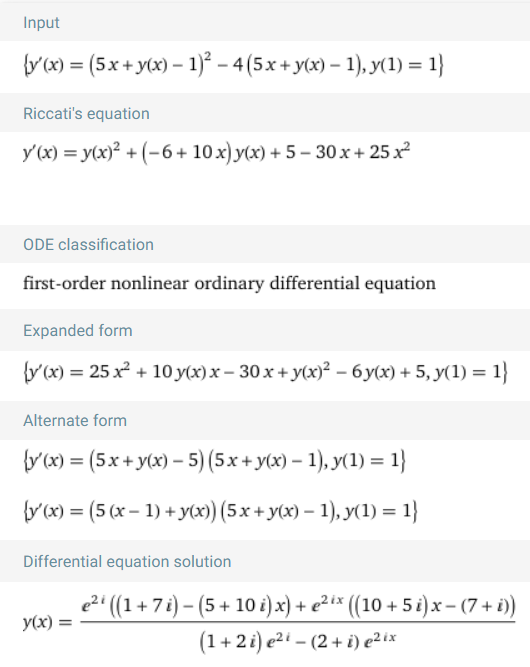
\includegraphics[width=0.8\textwidth]{wolfram_sol.png}
    \caption{Решение от Wolfram Alpha}
    \label{fig:wolfram_sol}
\end{figure}

\begin{FlushLeft}
То ни дава някакво решение, но изглежда не използва факта, че уравнението е доста нагласено и го свежда до уравнение на Рикати от вида $y' = a(x)y^2 + b(x)y + c(x)$, което не може да се реши в общия случай с елементарни математически операции. Wolfram ни дава някакво комплексно решение. Няма да го изследваме дали съвпада с нашето получено. Вместо това ще направим проверка за коректност на нашето решение по друг начин.

Ще проверим дали решението ни е коректно по по-традиционен начин, а именно като заместим с получения резултат и видим дали имаме тъждество. Вместо да го правим на ръка, това е добър момент да въведем символно смятане. В случая ще накараме машина (с помощта на Octave) да направи нужните сметки.

\end{FlushLeft}

Код:
\lstinputlisting[language=Octave]{symbolic.m}

Изход:
\begin{lstlisting}[language=Octave]
y(x) = (symfun) -5*x + tan(C + x) + 3
C = (sym) -1 + atan(3)
y(x) = (symfun) -5*x + tan(x - 1 + atan(3)) + 3
lhs = (sym)

     2                     
  tan (x - 1 + atan(3)) - 4

rhs = (sym)

     2                     
  tan (x - 1 + atan(3)) - 4

ans = (sym) True
\end{lstlisting}

\end{document}